%!TEX root = main.tex
\section{Precise Visual Querying\label{sec:precise}}
Visual analysis often reveal important anomalies or trends in the data\cite{Morton2014}. However, it is often challenging to find the appropriate piece of information to realize these insights.

\subsection{Motivating Example}
Astronomers from the The Dark Energy Survey (DES)\cite{Drlica-Wagner2017} are interested in finding anomalous time series to discover astrophysical transients (objects whose brightness changes dramatically as a function of time), such as supernova explosions or quasars. When trying to find celestial objects corresponding to supernovae, which have a specific pattern of brightness over time, scientists need to individually inspect the visualizations of each object until they find ones that match the pattern. With more than 400 million objects in their catalog, each having their own set of time series brightness measurement, the process of manually exploring a large number of visualizations is not only error-prone, but also overwhelming for scientists who do not have extensive knowledge about their dataset.  
% Intention driven task-based querying (Precise search)
\par The astronomy use case highlights a common challenge in exploratory data analysis (EDA). There is often a large space of possible visualizations that could be generated from a given dataset and manual search through this large collection is inefficient. Visualization authoring tools such as Tableau and Excel focusses on presenting one visualization at a time. There is no systematic way to create, compare, and query large collections of visualizations. 
%\par There has been many related work in this space varying different dimensions of possible visualizations, including visual encodings~\cite{showme}, data facets, . We will focus on  
\subsection{Effortless Data Exploration with \zv}
\par The challenges presented earlier points to a need for tools that enables users to create and search through large collections of visualizations. Therefore, we developed \zv a visual query system that allowed users to search through large collections of visualizations. \zv is built on top of a querying language called ZQL, which provides a mechanism for managing collections of visualizations\cite{Siddiqui}. Contrary prior work on visualization languages for specifying visual encodings of individual visualizations~\cite{Stolte2002,Wilkinson2005}, ZQL supports high-level queries over visualization collections, such as composing, sorting, filtering a collection of visualization. ZQL functionals and primitives can be constructed into rich and expressive query semantics, with functionalties including : 
\begin{itemize}
	\item Finding top-k visualizations whose y values are most or least similar from a queried visualization (e.g. Find other cities with sold price over time similar to Manhattan. Varying along \textsc{city} while keeping \textsc{x=time,y=AVG(price)} fixed.) 
	\item Comparing across a collection of visualizations by iterating over one or more x, y, z attributes while fixing other attributes (e.g. Find a y attribute that varies with time similarly how average price changes over time)
	\item Finding a pair of X and Y axes where two specific visualization instances differ the most. (e.g. For what pair of attributes does the products `stapler' and `chair' differ the most?)
\end{itemize}
\par Given a ZQL query, \zv parses the query into a graph of visual component nodes(containing visualization information, such as X, Y columns) and task nodes (common and user-defined primitives for processing visual components, such as sort-filter). \zv then performs query optimization to merge together multiple nodes, as well as reducing the processing time required for individual visualization components. Using the optimized query plan, the executor compiles visual nodes into SQL queries for retreiving the visualization data and postprocesses the result via the defined operations. 
\par While ZQL provides powerful mechanism for expressively specifying queries on large collections visualizations, writing ZQL queries can be daunting for novice users. Therefore, we extracted a typical workflow of visualization querying (finding top-k most similar visualization from a collection with fixed X,Y while varying Z) to allow users to formulate ZQL queries through interactions. The user can either directly input ZQL queries through a frontend table input or their frontend interactions is mapped into ZQL queries. The query results are rendered as a ranked list of visualizations in the Results panel in the frontend. \zv is a full-fledged visual querying system that supports a variety of querying interactions as illustrated in Figure~\ref{fig:modalities}. In the following section, we will discuss the design process of how we developed this visual query system and the lessons that we have learned for designing future visual data exploration systems.

\begin{figure}[h!]
\label{fig:modalities}
\centering
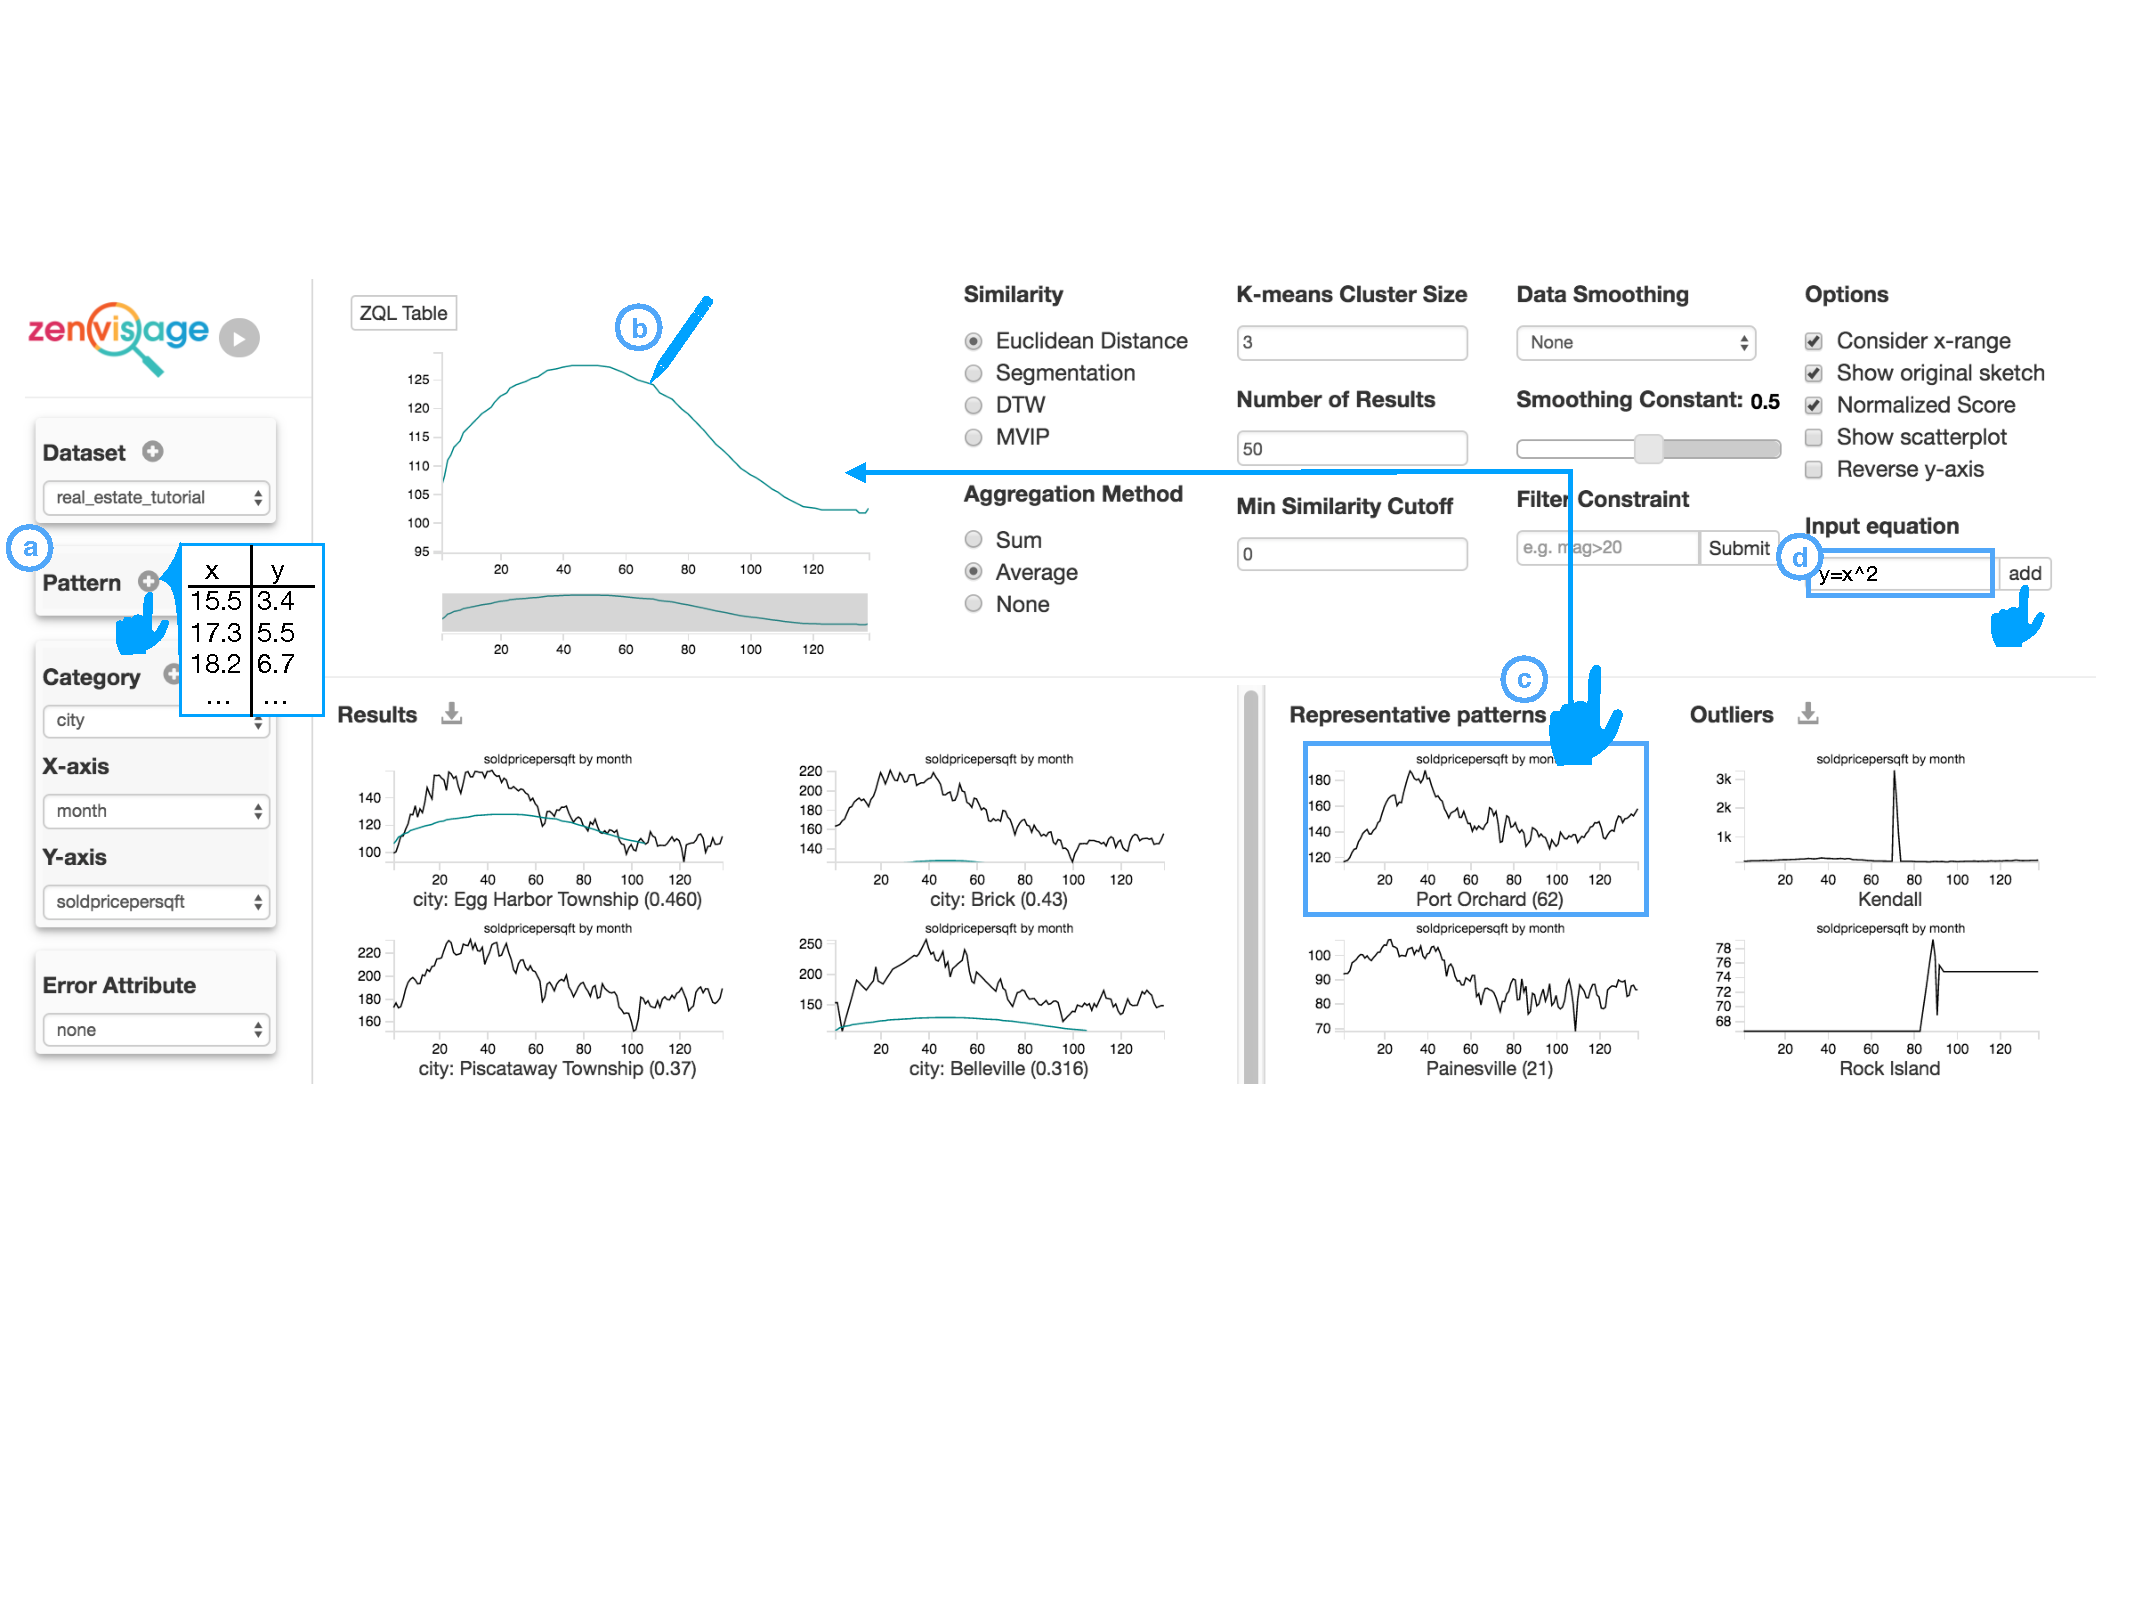
\includegraphics[width=0.8\textwidth]{figures/modalities.pdf}
\caption{\zv offers a variety of querying modalities, including: a) uploading a sample pattern from an external dataset as a query, b) sketching a query pattern, c) dragging-and-dropping an existing pattern from the dataset, and d) inputting an equation as a query.}
\end{figure}
